\chapter{Linux とは}
\label{chap:what_is_linux}

% この章で学ぶこと
\begin{goalbox}
  \begin{itemize}
    \item Linux が生まれた歴史と、その土台にある UNIX 哲学
    \item オープンソースソフトウェア（OSS）の考え方とライセンス
    \item ディストリビューションとは何か、Ubuntu のバージョンの読み方
    \item ロボット開発で Linux が使われる理由
    \item Ubuntu 環境の用意の仕方と、デスクトップ環境の基本操作
  \end{itemize}
\end{goalbox}

\ref{chap:computer}章では、コンピュータを管理する基本ソフトウェアとして OS を紹介しました。
この章では、本書で使う OS である \textbf{Linux} について、その成り立ちや考え方、そしてロボット開発で使われている理由を見ていきます。

\section{Linux の歴史と UNIX 哲学}
\label{sec:linux-history}

Linux は、ある日突然生まれたわけではありません。
その背景には、半世紀以上前に生まれた UNIX という OS と、ソフトウェアを自由に共有しようとした人々の歴史があります（図\ref{fig:linux-history}）。

\begin{figure}[tb]
  \centering
  % 図：UNIX から Linux への流れ（chapters/linux/what_is_linux.tex）
\begin{tikzpicture}[y=-0.75cm]
  \draw[thick, black!40] (1.4,-0.4) -- (1.4,7.4);
  \foreach \year/\text/\col [count=\i from 0] in {
      1969/UNIX 誕生（AT\&T ベル研究所）/black,
      1970 年代/BSD など UNIX の派生版が広がる/black,
      1983/GNU プロジェクト開始/green!50!black,
      1991/Linux カーネル公開（Linus Torvalds）/blue!70!black,
      1992/Linux カーネルが GPL で配布されるように/blue!70!black,
      2004/Ubuntu の最初のバージョンが公開/orange!80!black,
      2008/Linux カーネルを使った Android 端末が登場/blue!70!black,
      2024/Ubuntu 24.04 LTS 公開/orange!80!black} {
    \fill[\col] (1.4,\i) circle (1.2mm);
    \node[anchor=east, font=\small\bfseries] at (1.15,\i) {\year};
    \node[anchor=west, font=\small, text=\col] at (1.65,\i) {\text};
  }
\end{tikzpicture}

  \caption{UNIX から Linux への流れ}
  \label{fig:linux-history}
\end{figure}

\subsection{UNIX の誕生}

1969 年、アメリカの AT\&T ベル研究所で、Ken Thompson と Dennis Ritchie らによって \textbf{UNIX} という OS が作られました。
UNIX は、その後 C 言語で書き直されたことで、さまざまなコンピュータに移植しやすくなりました。
大学や研究機関にも広く配られ、カリフォルニア大学バークレー校で作られた BSD をはじめ、多くの派生版が生まれました。

一方で、UNIX は企業の製品でもあったため、次第にソースコードを自由に読んだり改良したりすることが難しくなっていきました。

\subsection{GNU プロジェクト}

こうした状況に対して、1983 年に Richard Stallman が始めたのが \textbf{GNU プロジェクト}です。
GNU は「GNU's Not UNIX」の略で、UNIX と同じように使えて、誰もが自由に使い、改良し、共有できる OS を一から作ることを目指しました（この考え方については\ref{sec:linux-oss}節で詳しく説明します）。

GNU プロジェクトは、コンパイラ（GCC）やシェル（bash）、エディタ（Emacs）、さまざまなコマンドなど、OS を構成するソフトウェアを次々に作っていきました。
しかし、OS の中心となる\textbf{カーネル}（ハードウェアを直接管理する部分）の開発は難航していました。

\subsection{Linux の誕生}

1991 年、フィンランドのヘルシンキ大学の学生だった \textbf{Linus Torvalds} は、趣味として自分のパソコンで動く OS のカーネルを作り始めました。
Torvalds はそのソースコードをインターネット上で公開し、ほかの開発者に意見や協力を求めました。
これが \textbf{Linux} カーネルの始まりです。

Linux カーネルは、1992 年に GNU の GPL ライセンス（\ref{sec:linux-oss}節）で配布されるようになりました。
GNU プロジェクトが作ってきたソフトウェアと Linux カーネルを組み合わせることで、誰もが自由に使える UNIX のような OS がついに完成したのです。
その後、Linux はインターネットを通じて世界中の開発者の協力を得て、急速に成長していきました。

\begin{point}[「Linux」という言葉の 2 つの意味]
  厳密には、Linux は OS の中心部分である\textbf{カーネル}だけを指す名前です。
  しかし一般には、Linux カーネルに GNU のソフトウェアなどを組み合わせた OS 全体を「Linux」と呼ぶことがほとんどです。
  本書でも、特に断らない限り、OS 全体を指して Linux と呼びます。
  なお、GNU プロジェクトの貢献を明確にするため、OS 全体を「GNU/Linux」と呼ぶ人もいます。
\end{point}

\subsection{現在の Linux}

現在、Linux は私たちの身の回りのあらゆるところで使われています。

\begin{itemize}
  \item インターネット上の Web サーバやクラウドサービスの多く
  \item 世界の最先端のスーパーコンピュータ（性能上位のほぼすべて）
  \item スマートフォンの Android（Linux カーネルを使っています）
  \item テレビや家電、自動車などの組込み機器
  \item そして、多くのロボット
\end{itemize}

パソコン用の OS としては Windows や macOS に比べて利用者は少ないものの、コンピュータの世界全体で見れば、Linux は最も広く使われている OS の 1 つです。

\subsection{UNIX 哲学}

UNIX の開発者たちは、ソフトウェアをどのように作るべきかについて、ある共通の考え方を持っていました。
これは \textbf{UNIX 哲学}と呼ばれ、UNIX の流れをくむ Linux にも受け継がれています。
UNIX 哲学にはいくつかの表現がありますが、よく知られているのは Doug McIlroy による次の言葉です。

\begin{enumerate}
  \item 1 つのことをうまくやるプログラムを書け
  \item 協調して動くプログラムを書け
  \item テキストを扱うプログラムを書け。テキストは万能のインターフェースだからである
\end{enumerate}

たとえば Linux には、「ファイルの一覧を表示する」「文字列を検索する」「行を並べ替える」「行数を数える」といった、それぞれ 1 つの仕事だけをする小さなコマンドがたくさんあります。
これらのコマンドは、テキストを受け渡すことで組み合わせて使えるようになっていて、小さな部品を組み合わせることで複雑な処理を実現できます（\ref{chap:text_pipe}章で扱うパイプ）。
また、デバイスなどもファイルとして扱う「すべてはファイル」という考え方も、UNIX から受け継がれたものです（\ref{chap:linux_internals}章）。

\begin{column}{ROS と UNIX 哲学}
  実は、本書の後半で学ぶ ROS 2 の設計にも、UNIX 哲学に通じる考え方が見られます。
  ROS 2 では、「カメラの画像を取得する」「画像から物体を見つける」「モータを制御する」といった 1 つ 1 つの機能を、\textbf{ノード}という小さなプログラムとして作ります。
  そして、ノード同士がメッセージをやり取りすることで、ロボット全体として複雑な動きを実現します（\ref{chap:ros2_concepts}章）。
  「小さな部品を作り、それらを組み合わせる」という考え方を身につけておくと、ROS 2 の理解にも役立ちます。
\end{column}

\section{オープンソースソフトウェア}
\label{sec:linux-oss}

Linux カーネルは、世界中の誰でもソースコード（プログラムの設計図にあたる文字）を読むことができ、自由に改良して配ることもできます。
このように、ソースコードが公開され、誰でも利用・改良・再配布できるソフトウェアを\textbf{オープンソースソフトウェア}（Open Source Software、\textbf{OSS}）といいます。
Linux だけでなく、本書で扱う Ubuntu、Git、Python、ROS 2、Gazebo も、すべて OSS です。
ロボット開発の世界を理解するうえで、OSS の考え方は欠かせません。

\subsection{ソースコードが公開されているということ}

一般的な市販のソフトウェアは、コンピュータが実行できる形（実行ファイル）だけが配られ、ソースコードは公開されていません。
使うことはできても、中でどのような処理をしているのかを確かめたり、不具合を自分で直したりすることはできません。

これに対して OSS では、ソースコードが公開されています。
そのため、利用者は次のようなことができます。

\begin{itemize}
  \item 中身を読んで、どのように動いているのかを学ぶ
  \item 不具合を見つけたら、自分で原因を調べて直す
  \item 自分の目的に合わせて機能を追加する
  \item 改良したものを、ほかの人にも配る
\end{itemize}

ロボット開発では、センサのドライバや制御のアルゴリズムが「思ったとおりに動かない」ことがよくあります。
そのようなとき、ソースコードを読んで原因を突き止められることは、OSS の大きな強みです。

\subsection{フリーソフトウェアとオープンソース}

ソフトウェアを自由に共有しようという考え方は、1980 年代に始まった\textbf{フリーソフトウェア}運動にさかのぼります。
Richard Stallman は 1983 年に GNU プロジェクトを始め、利用者に次の 4 つの自由を保障するソフトウェアを「フリーソフトウェア」と呼びました。

\begin{enumerate}
  \item 目的を問わず、プログラムを実行する自由
  \item プログラムがどのように動いているかを調べ、改変する自由（そのためにソースコードを入手できること）
  \item コピーを再配布する自由
  \item 改変したものを配布する自由
\end{enumerate}

ここでいう「フリー」は「無料」ではなく「自由」を意味します。
その後 1998 年に、この考え方を企業などにも受け入れられやすい形で広めるため、「オープンソース」という言葉が生まれました。
2 つの言葉は重視する点が少し異なりますが、対象となるソフトウェアの多くは共通しています。

\begin{point}[OSS は「無料のソフトウェア」ではない]
  OSS の多くは無料で入手できますが、OSS の本質は価格ではなく、ソースコードを読み、改良し、共有する自由にあります。
  逆に、無料で配られていてもソースコードが公開されていないソフトウェア（フリーウェア）は OSS ではありません。
\end{point}

\subsection{ライセンス}

OSS だからといって、どのように使ってもよいわけではありません。
OSS には、利用・改変・再配布の条件を定めた\textbf{ライセンス}が付いています。
代表的なライセンスには、次のようなものがあります。

\begin{center}
  \begin{tabular}{lp{0.65\linewidth}}
    \toprule
    ライセンス & 特徴 \\
    \midrule
    GPL & 改変したものを配布するときは、同じ GPL でソースコードも公開しなければならない（Linux カーネル、Git など） \\
    MIT & 著作権表示とライセンス文を残せば、ほぼ自由に利用できる \\
    BSD & MIT とほぼ同様。著作権者の名前を宣伝に使うことを禁じるものもある \\
    Apache 2.0 & MIT に近い自由さに加え、特許の扱いを明確にしている（ROS 2、Gazebo など） \\
    \bottomrule
  \end{tabular}
\end{center}

GPL のように、改変したものにも同じ自由を引き継がせるライセンスを\textbf{コピーレフト}型、MIT や Apache 2.0 のように条件がゆるやかなライセンスを\textbf{パーミッシブ}型と呼びます。

\begin{caution}[他人のコードを使うときはライセンスを確認する]
  インターネット上で見つけたコードを自分のプログラムに取り込むときは、必ずライセンスを確認してください。
  特に、ライセンスが書かれていないコードは、公開されていても自由に使ってよいとは限りません（著作権は作者にあるため、原則として作者の許可が必要です）。
  自分でコードを公開するときも、ほかの人が安心して使えるようにライセンスを明記しましょう。
  ROS 2 のパッケージでは、\cmd{package.xml} にライセンスを書きます（\ref{chap:workspace}章）。
\end{caution}

\subsection{コミュニティによる開発}

OSS の多くは、特定の会社の中だけでなく、世界中の開発者が参加する\textbf{コミュニティ}によって開発されています。
Linux カーネルも、1991 年に Linus Torvalds が個人で公開したものが、インターネットを通じて多くの開発者の協力を得て育ってきました。
現在では、個人のボランティアだけでなく、多くの企業も開発に参加しています。

OSS の開発には、誰でも参加できます。
参加の方法は、プログラムを書くことだけではありません。

\begin{itemize}
  \item 不具合を見つけて報告する
  \item ドキュメントの誤りを直したり、翻訳したりする
  \item 使い方の質問に答える
  \item 機能を改良して、その変更を取り込んでもらうよう提案する
\end{itemize}

\begin{figure}[tb]
  \centering
  % 図：Issue と Pull Request による OSS 開発の流れ（chapters/linux/what_is_linux.tex）
\begin{tikzpicture}
  
  \foreach \a/\name/\text in {
      90/use/利用者がソフトウェアを使う,
      18/issue/不具合を見つけて\\Issue で報告,
      -54/pr/誰かが修正して\\Pull Request を送る,
      -126/review/レビューを経て\\変更が取り込まれる,
      162/release/新しい版が\\公開される} {
    \node[figpart, minimum width=26mm, font=\footnotesize] (\name) at (\a:2.9cm and 2.3cm) {\text};
  }
  \foreach \a/\b in {use/issue, issue/pr, pr/review, review/release, release/use}
    \draw[figarrow] (\a) to[bend left=18] (\b);
  \node[figlabel, text=black!60] at (0,0) {GitHub など};
\end{tikzpicture}

  \caption{Issue と Pull Request による OSS 開発の流れ}
  \label{fig:linux-oss-community}
\end{figure}

こうした開発の多くは、GitHub などのサービス上で、Issue（課題の報告）や Pull Request（変更の提案）という形で行われます（\ref{chap:git}章）。
図\ref{fig:linux-oss-community}に、OSS が改良されていく流れを示します。

\subsection{ロボット開発と OSS}

ロボットを動かすには、センサからのデータの取得、地図の作成、経路の計画、モータの制御など、たくさんのソフトウェアが必要です。
これらをすべて自分たちだけで一から作るのは、現実的ではありません。

ROS は、世界中の研究者や開発者が作ったソフトウェアを OSS として共有し、組み合わせて使えるようにすることで、この問題を解決してきました。
誰かが作った地図作成のパッケージを別の誰かが改良し、それをまた別の誰かが自分のロボットで使う、という積み重ねによって、ロボット開発は大きく進歩してきたのです（\ref{chap:what_is_ros}章）。
本書の最後の\ref{chap:practice}章で体験する SLAM や自律移動も、こうした OSS の成果です。

本書を読み進めるあなたも、最初は OSS を使う側ですが、いずれは不具合の報告や改良の提案を通じて、OSS を育てる側の一員になることができます。

\begin{column}{Ubuntu と OSS のビジネス}
  「無料で配って、どうやって開発を続けているのだろう？」と疑問に思うかもしれません。
  たとえば Ubuntu は、Canonical という会社が中心となって開発しています。
  Canonical は、Ubuntu そのものは無料で配布しながら、企業向けの長期サポートやクラウド向けのサービスなどで収益を得ています。
  このように、OSS を中心にしたビジネスも数多く成り立っています。
\end{column}

\section{ディストリビューション}
\label{sec:linux-distribution}

Linux カーネルだけでは、コンピュータを便利に使うことはできません。
実際に使うには、カーネルに加えて、コマンドやライブラリ、デスクトップ環境、アプリケーション、そしてソフトウェアをインストールするためのしくみなどが必要です。
これらをまとめて、すぐに使える形で配布しているものを \textbf{ディストリビューション}（distribution、略して\textbf{ディストロ}）といいます（図\ref{fig:linux-distribution}）。

\begin{figure}[tb]
  \centering
  % 図：ディストリビューションの構成（chapters/linux/what_is_linux.tex）
\begin{tikzpicture}
  \node[figpart, minimum width=62mm, fill=blue!18] (kernel) at (0,0) {\textbf{Linux カーネル}};
  \node[figbox, minimum width=62mm, fill=blue!6, above=2mm of kernel] (gnu) {GNU のコマンド・ライブラリ};
  \node[figbox, minimum width=30mm, fill=green!6, above=2mm of gnu.north west, anchor=south west] (desk) {デスクトップ環境\\{\footnotesize（GNOME など）}};
  \node[figbox, minimum width=30mm, fill=green!6, above=2mm of gnu.north east, anchor=south east] (apps) {アプリケーション\\{\footnotesize（ブラウザなど）}};
  \node[figbox, minimum width=24mm, fill=orange!8, right=3mm of kernel.south east, anchor=south west, minimum height=12mm] (pkg) {パッケージ\\管理システム\\{\footnotesize（apt など）}};
  \node[figbox, minimum width=24mm, fill=orange!8, above=2mm of pkg, minimum height=12mm] (inst) {インストーラ};
  \begin{scope}[on background layer]
    \node[draw, thick, rounded corners=4pt, fill=black!3, inner sep=4mm,
      fit=(kernel)(gnu)(desk)(apps)(pkg)(inst), label={[font=\small\bfseries]above:ディストリビューション（Ubuntu など）}] {};
  \end{scope}
\end{tikzpicture}

  \caption{ディストリビューションの構成}
  \label{fig:linux-distribution}
\end{figure}

Linux カーネルと多くのソフトウェアは OSS なので、誰でも自由に組み合わせてディストリビューションを作ることができます。
そのため、世界には数百ものディストリビューションが存在します。
ディストリビューションごとに、対象とする利用者や、ソフトウェアの更新の方針、標準の見た目などが異なります。

\subsection{主なディストリビューション}

ディストリビューションは、元になったディストリビューションによっていくつかの系統に分けられます。
同じ系統のディストリビューションは、ソフトウェアのインストール方法（\textbf{パッケージ管理システム}）などが共通しています（\ref{chap:package}章）。

\begin{center}
  \begin{tabular}{lp{0.6\linewidth}}
    \toprule
    系統 & 主なディストリビューションと特徴 \\
    \midrule
    Debian 系 & Debian、Ubuntu、Linux Mint、Raspberry Pi OS など。\cmd{apt} コマンドでソフトウェアを管理する \\
    Red Hat 系 & Red Hat Enterprise Linux、Fedora、Rocky Linux など。\cmd{dnf} コマンドでソフトウェアを管理する。企業のサーバで多く使われる \\
    その他 & Arch Linux、openSUSE など \\
    \bottomrule
  \end{tabular}
\end{center}

\subsection{Ubuntu}

本書では、Debian 系のディストリビューションである \textbf{Ubuntu} を使います。
Ubuntu は、Canonical 社が中心となって開発しているディストリビューションで、2004 年に最初のバージョンが公開されました。
初心者にも使いやすいことを目標にしていて、デスクトップ用としてもサーバ用としても、世界で最も広く使われているディストリビューションの 1 つです。
利用者が多いため、困ったときにインターネット上で情報を見つけやすいのも大きな利点です。

\subsection{Ubuntu のバージョン}

Ubuntu のバージョン番号は、リリースされた年の下 2 桁と月を \cmd{.} でつないだものです。
たとえば、本書で使う \textbf{Ubuntu 24.04} は、2024 年 4 月にリリースされたバージョンです。
Ubuntu は毎年 4 月と 10 月の 2 回、新しいバージョンがリリースされます。

また、各バージョンには、形容詞と動物の名前を組み合わせたコードネームが付いています。
コードネームの頭文字は、バージョンが上がるごとにアルファベット順に進んでいきます。

\begin{center}
  \begin{tabular}{lll}
    \toprule
    バージョン & コードネーム & 対応する主な ROS 2 \\
    \midrule
    Ubuntu 20.04 LTS & Focal Fossa & ROS 2 Foxy（サポート終了） \\
    Ubuntu 22.04 LTS & Jammy Jellyfish & ROS 2 Humble \\
    Ubuntu 24.04 LTS & Noble Numbat & ROS 2 Jazzy \\
    \bottomrule
  \end{tabular}
\end{center}

コマンドやインターネット上の情報では、\cmd{noble} や \cmd{jammy} のように、コードネームの最初の単語を小文字にしてバージョンを表すことがよくあります。

\subsection{LTS 版}

2 年に 1 度、偶数年の 4 月にリリースされるバージョンは \textbf{LTS}（Long Term Support、長期サポート）版と呼ばれます。
LTS 版は 5 年間にわたって、セキュリティの修正などのアップデートが提供されます（Ubuntu Pro を使うと、さらに延長できます）。
それ以外のバージョンのサポート期間は 9 か月しかありません。

ロボットのように、一度環境を整えたら長く安定して使い続けたい用途では、LTS 版を使うのが基本です。
ROS 2 の主要なバージョンも、Ubuntu の LTS 版に合わせてリリースされています（\ref{chap:what_is_ros}章）。
本書で使う ROS 2 Jazzy は、Ubuntu 24.04 LTS で動かすことを前提に作られているため、本書でも Ubuntu 24.04 LTS を使います。

\begin{caution}[Ubuntu と ROS 2 のバージョンの組み合わせ]
  ROS 2 のバージョンごとに、対応する Ubuntu のバージョンが決まっています。
  たとえば、ROS 2 Jazzy を Ubuntu 22.04 にインストールすることは、公式にはサポートされていません。
  インターネット上の情報を参考にするときは、それがどの Ubuntu と ROS 2 の組み合わせで書かれたものかを確認するようにしましょう。
\end{caution}

\section{なぜロボット開発で Linux が使われるのか}
\label{sec:linux-why-robot}

パソコンでは Windows や macOS を使っている人が多いのに、なぜロボット開発では Linux が使われるのでしょうか。
主な理由は、次のとおりです。

\subsection{ROS 2 が Linux を中心に開発されている}

最も直接的な理由は、ロボット開発で広く使われている ROS 2 が、Linux（特に Ubuntu）を中心に開発・テストされていることです。
ROS 2 は Windows や macOS でも動かせるように作られていますが、最も手厚くサポートされているのは Ubuntu です。
ROS 2 の上で公開されている多くのパッケージも Ubuntu での利用を前提としており、公式のドキュメントや解説記事の多くも Ubuntu を使って書かれています。

\subsection{オープンソースで自由に使える}

\ref{sec:linux-oss}節で説明したように、Linux は OSS です。
無料で使えるうえ、ソースコードを読んで動きを確かめたり、ロボットに合わせて改良したりできます。
画像処理の OpenCV、点群処理の PCL、シミュレータの Gazebo など、ロボット開発で使われる多くのソフトウェアも OSS として Linux 向けに提供されています。

\subsection{さまざまなハードウェアで動く}

Linux は、一般的なパソコンだけでなく、Raspberry Pi のようなシングルボードコンピュータや、NVIDIA Jetson のような GPU を搭載した組込み向けコンピュータでも動きます（\ref{sec:computer-robot}節）。
開発用のパソコンで作ったプログラムを、ほぼそのままロボットに載せたコンピュータで動かせるのは、大きな利点です。
また、不要な機能を省いて軽く動かすこともできるので、性能や電力が限られたロボットのコンピュータにも向いています。

\subsection{画面がなくても操作しやすい}

Linux は、もともとサーバのように画面のないコンピュータで使われることが多かったため、CLI でほとんどすべての操作ができるようになっています。
ロボットに載せたコンピュータにモニタやキーボードをつながなくても、ネットワーク越しに別のコンピュータから操作できます（\ref{chap:network}章）。

\subsection{センサやモータを扱いやすい}

Linux では、USB でつないだセンサやモータのコントローラなどのデバイスを、ファイルと同じように読み書きできます（\ref{chap:linux_internals}章）。
デバイスを扱うためのドライバやツールも豊富で、ロボットのハードウェアをプログラムから直接扱いやすくなっています。
また、決められた時間内に確実に処理を行う\textbf{リアルタイム性}が求められる場面に向けて、そのための機能も用意されています。

\subsection{開発のための道具と情報が充実している}

Linux には、プログラミング言語の開発環境、バージョン管理システムの Git、コンテナ技術の Docker など、ソフトウェア開発に必要な道具が揃っています（第III部）。
ロボットに限らず、サーバやクラウド、AI の分野でも Linux が標準的に使われているため、ここで身につけた Linux の知識は、ロボット開発以外の場面でも役に立ちます。

\begin{point}[Windows や macOS を使っている人へ]
  ふだん Windows や macOS を使っている人も、Linux のためにパソコンを買い替える必要はありません。
  仮想マシンや WSL2、Docker などを使えば、今のパソコンの上で Ubuntu を動かすことができます。
  具体的な方法は、次の\ref{sec:linux-setup}節で説明します。
\end{point}

\section{Ubuntu 環境の用意}
\label{sec:linux-setup}

本書の内容を実際に試すには、Ubuntu 24.04 が動く環境が必要です。
ここでは、Ubuntu の環境を用意するいくつかの方法を紹介し、その中から自分に合った方法を選べるようにします。

\subsection{環境を用意する方法}

Ubuntu の環境を用意する方法には、主に次のようなものがあります。

\begin{center}
  \begin{tabular}{lp{0.3\linewidth}p{0.3\linewidth}}
    \toprule
    方法 & 良いところ & 気になるところ \\
    \midrule
    専用の PC にインストール & 性能を最大限に使え、トラブルが最も少ない & PC が 1 台必要 \\
    デュアルブート & 1 台の PC で Windows と使い分けられる & 起動のたびに OS を選ぶ。設定を誤ると既存のデータを失うおそれ \\
    仮想マシン & 今の OS の上で手軽に試せる & 動作が遅く、GPU や USB 機器の扱いに制限がある \\
    WSL2 & Windows の上で手軽に使える & USB 機器やネットワークの扱いに追加の設定が必要 \\
    Docker & 環境を丸ごと再現・共有できる & しくみの理解が必要（\ref{chap:docker}章） \\
    \bottomrule
  \end{tabular}
\end{center}

ロボットを実際に動かすことを考えると、\textbf{Ubuntu を専用の PC にインストールする}方法が最もおすすめです。
センサやモータを USB でつないだり、シミュレータで 3D の描画をしたりするときに、ほかの方法では思わぬ制限にぶつかることがあるからです。
古いノートパソコンなどを 1 台、Ubuntu 専用にできると理想的です。
まずは手元の PC で試してみたいという場合は、仮想マシンや WSL2 から始めても構いません。

PC の性能の目安は、次のとおりです。
シミュレータ（\ref{chap:simulation}章）を快適に動かすには、これより余裕があると安心です。

\begin{itemize}
  \item CPU：4 コア以上
  \item メモリ：8 GB 以上（16 GB 以上を推奨）
  \item ストレージ：空き容量 50 GB 以上
\end{itemize}

\subsection{PC に Ubuntu をインストールする}

PC に Ubuntu をインストールする流れは、おおむね次のとおりです。

\begin{enumerate}
  \item \textbf{インストール用のファイルを入手する}：
    Ubuntu の公式サイト（\url{https://jp.ubuntu.com/download} など）から、Ubuntu 24.04 LTS のデスクトップ版のファイル（拡張子が \cmd{.iso} のファイル）をダウンロードします。
  \item \textbf{インストール用の USB メモリを作る}：
    8 GB 以上の USB メモリに、balenaEtcher や Rufus といったツールを使ってダウンロードしたファイルを書き込みます。
    USB メモリの中身はすべて消えるので注意してください。
  \item \textbf{USB メモリから起動する}：
    インストールしたい PC に USB メモリを差して電源を入れ、起動するときに特定のキー（\key{F12} や \key{F2} など、機種によって異なります）を押して、USB メモリから起動します。
  \item \textbf{インストーラの指示に従う}：
    言語（日本語）、キーボードの配列、ネットワーク、インストールの種類などを選びます。
    ディスクの設定で「ディスクを削除して Ubuntu をインストール」を選ぶと、その PC の中のデータはすべて消えます。
  \item \textbf{ユーザを作る}：
    自分の名前、コンピュータの名前（ホスト名、\ref{sec:terminal-prompt}節）、ユーザ名、パスワードを設定します。
    ユーザ名とホスト名は、ターミナルで何度も目にすることになるので、半角英小文字の短い名前にしておくと便利です。
  \item \textbf{再起動する}：
    インストールが終わったら USB メモリを抜いて再起動し、設定したユーザでログインします。
\end{enumerate}

\begin{caution}[インストールの前にバックアップを]
  Ubuntu のインストールでは、ディスクの設定を誤ると、PC の中のデータがすべて消えてしまいます。
  特にデュアルブートにする場合は、インストールの前に、大切なデータを必ず別の場所にバックアップしておきましょう。
\end{caution}

インストールが終わったら、最初にソフトウェアを最新の状態に更新しておきます。
ターミナル（\ref{chap:terminal_shell}章）を開いて、次のコマンドを実行します（\ref{chap:package}章で詳しく説明します）。

\begin{terminal}[インストール後にソフトウェアを更新する]
$ sudo apt update
$ sudo apt upgrade
\end{terminal}

NVIDIA の GPU を搭載した PC では、「ソフトウェアとアップデート」の「追加のドライバー」から、NVIDIA のドライバをインストールしておくと、3D の描画が快適になります。

\subsection{仮想マシン・WSL2 で使う}

\textbf{仮想マシン}を使う場合は、VirtualBox や VMware Workstation などのソフトウェアをインストールし、ダウンロードした Ubuntu の \cmd{.iso} ファイルを使って、仮想マシンの中に Ubuntu をインストールします。
Apple シリコン（M1 など）を搭載した Mac では、UTM や Parallels Desktop などを使って、ARM 版の Ubuntu をインストールします。
仮想マシンには、メモリを 8 GB 程度、CPU を 4 コア程度割り当てると、ROS 2 の学習には十分です。

Windows 11 の PC では、\textbf{WSL2}（Windows Subsystem for Linux）を使うと、Windows の中で Ubuntu を手軽に使えます。
管理者として開いた PowerShell で、次のコマンドを実行すると、Ubuntu 24.04 がインストールされます。

\begin{terminal}[WSL2 で Ubuntu 24.04 をインストールする（PowerShell）]
PS> wsl --install -d Ubuntu-24.04
\end{terminal}

WSL2 では、Linux の GUI アプリを Windows の画面に表示することもできるので、本書の内容の多くを試せます。
ただし、USB でつないだ機器を使うには追加のツールが必要など、実機のロボットを動かすには不便な点もあります。

\section{デスクトップ環境の基本操作}
\label{sec:linux-desktop}

Ubuntu 24.04 には、\textbf{GNOME}（グノーム）という\textbf{デスクトップ環境}が採用されています。
デスクトップ環境とは、ウィンドウやアイコン、メニューなど、マウスで操作するための画面（GUI、\ref{sec:terminal-gui-cui}節）を提供するソフトウェアです。
ログインすると、図\ref{fig:linux-desktop}のような画面が表示されます。

\begin{figure}[tb]
  \centering
  \large
  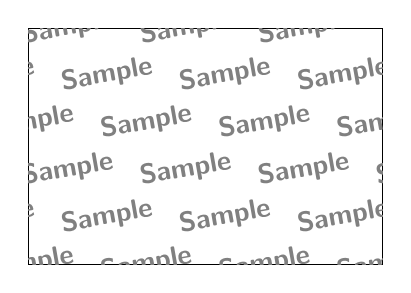
\begin{tikzpicture}
    \draw rectangle++(4.5,3);
    \clip rectangle++(4.5,3);
    \foreach\x in{0,1,2,3,4}{
      \foreach\y in{0,1,2,3,4,5,6}{
        \path(\x*1.5-\y*0.5,\y*0.6)node[rotate=10,text=gray]{\sffamily\bfseries\itshape Sample };
      }
    }
  \end{tikzpicture}
  %% 入れる画像：Ubuntu 24.04 にログインした直後のデスクトップ画面のスクリーンショット（上部バー、左側の Dock、アプリ一覧のボタンに番号を付ける）
  % eps 画像を貼る場合は includegraphics をお使いください。
  % \includegraphics[width=0.8\linewidth]{what_is_linux/desktop.png}
  \caption{Ubuntu 24.04 のデスクトップ}
  \label{fig:linux-desktop}
\end{figure}

\subsection{画面の構成}

\begin{description}
  \item[上部バー]
    画面の上端にあるバーです。
    左端の「アクティビティ」を押すと、開いているウィンドウの一覧と検索画面が表示されます。
    中央には日付と時刻が、右端には、ネットワークや音量、電源などを操作するシステムメニューがあります。
  \item[Dock]
    画面の左端に並んでいるアイコンです。
    よく使うアプリケーションを起動したり、起動中のアプリケーションを切り替えたりできます。
    一番下のボタンを押すと、インストールされているすべてのアプリケーションの一覧が表示されます。
  \item[ワークスペース]
    仮想的な画面を複数用意して、作業ごとに使い分けるしくみです。
    たとえば、1 つ目のワークスペースでエディタとターミナルを、2 つ目のワークスペースでシミュレータを開く、といった使い方ができます。
\end{description}

\subsection{よく使うアプリケーション}

\begin{description}
  \item[ファイル] ファイルやディレクトリを GUI で操作するファイルマネージャです（\ref{sec:terminal-gui-cui}節）。
  \item[端末] コマンドを入力するためのターミナルです（\ref{chap:terminal_shell}章）。本書で最もよく使うアプリケーションです。
  \item[設定] ネットワーク（Wi-Fi）、ディスプレイ、キーボード、言語、ユーザなどの設定を行います。
  \item[App Center] アプリケーションを検索してインストールできます（\ref{chap:package}章）。
  \item[Firefox] Web ブラウザです。
\end{description}

\subsection{便利なショートカットキー}

キーボードの \key{Super} キーは、Windows のロゴが描かれたキーのことです。
次のショートカットキーを覚えておくと、マウスを使わずに素早く操作できます。

\begin{center}
  \begin{tabular}{ll}
    \toprule
    キー & 動作 \\
    \midrule
    \key{Super} & アクティビティ画面を開く（続けて文字を入力するとアプリを検索できる） \\
    \key{Ctrl}+\key{Alt}+\key{T} & ターミナルを開く \\
    \key{Alt}+\key{Tab} & ウィンドウを切り替える \\
    \key{Super}+\key{\(\leftarrow\)} / \key{\(\rightarrow\)} & ウィンドウを画面の左半分 / 右半分に配置する \\
    \key{Super}+\key{\(\uparrow\)} & ウィンドウを最大化する \\
    \key{Super}+\key{L} & 画面をロックする \\
    \key{Print} & スクリーンショットを撮る \\
    \bottomrule
  \end{tabular}
\end{center}

ターミナルとエディタを画面の左右に並べて作業することが多いので、\key{Super}+\key{\(\leftarrow\)} / \key{\(\rightarrow\)} は特に便利です。

\begin{point}[日本語の入力]
  日本語を選んでインストールした場合、日本語入力のソフトウェア（Mozc）も使えるようになっています。
  日本語入力と英字入力は、\key{半角/全角} キーで切り替えます。
  ターミナルでコマンドを入力するときは、英字入力になっているかを確かめましょう。
  全角の文字やスペースが混ざると、コマンドは正しく動きません（\ref{sec:terminal-command-structure}節）。
\end{point}

\section*{この章のまとめ}

\begin{itemize}
  \item Linux は、1991 年に Linus Torvalds が公開したカーネルに、GNU プロジェクトのソフトウェアなどを組み合わせた、UNIX の流れをくむ OS です。
  \item 「1 つのことをうまくやる小さなプログラムを組み合わせる」という UNIX 哲学は、Linux のコマンドや ROS 2 の設計にも通じています。
  \item Linux は OSS であり、ソースコードを読み、改良し、共有する自由があります。他人のコードを使うときはライセンスを確認します。
  \item Linux カーネルにさまざまなソフトウェアを組み合わせて配布しているものをディストリビューションといいます。本書では Ubuntu 24.04 LTS を使います。
  \item ROS 2 が Ubuntu を中心に開発されていること、さまざまなハードウェアで動くこと、リモートから操作しやすいことなどから、ロボット開発では Linux が広く使われています。
  \item Ubuntu の環境は、専用の PC にインストールするのがおすすめです。手軽に試すなら、仮想マシンや WSL2 も使えます。
  \item Ubuntu 24.04 のデスクトップ環境は GNOME です。\key{Super} キーでアプリを検索し、\key{Ctrl}+\key{Alt}+\key{T} でターミナルを開きます。
\end{itemize}
